
\subsection{Answers}
\begin{table}[htb]%
\begin{center}%
\caption{Q13: Why did you choose the MPI implementation(s)? [Select most suitable one]}%
\label{tab:Q13-ans}%
\begin{tabular}{l|l|r}%
\hline%
Choice & Abbrv. & \# Answers \\%
\hline%
{\small I could not have any choice (the one pro$\cdots$} & No choice & 306 (36.4\%) \\%
I have no special reason. & No reason & 187 (22.3\%) \\%
I am familiar with it. & Familiar & 159 (18.9\%) \\%
I like to use it. & I like & 116 (13.8\%) \\%
I was said to use it. & Said to use & 72 (8.6\%) \\%
\hline%
\multicolumn{2}{c}{total} & 840 \\%
\hline%
\end{tabular}%
\end{center}%
\end{table}%


It is also interesting to see how the selection of the used MPI implementation has been decided or imposed. This highlights on one side who can impose the usage of a specific MPI implementation and how much leverage the final users can have on this choice. It is interesting to note the the overall distribution of the answers matches relatively well on all regions, indicating a well defined strategy for selecting the available/used MPI library. Moreover, if we split the answers into users making a willing choice on their MPI implementation and being imposed one (for any reason), it become clear than less than 20\% of users have been actively involved in the selection process of the available MPI library.
%
In a perfect setting where all libraries are equivalent in capabilities and performance such a low percentage of user involvement would not be problematic, as its impact on the scientific and engineering throughput would, at best, marginally impacted by the users choice. However, it is not clear we have reached such a leveled state in the MPI implementations yet.

\begin{figure}[htb]
\begin{center}
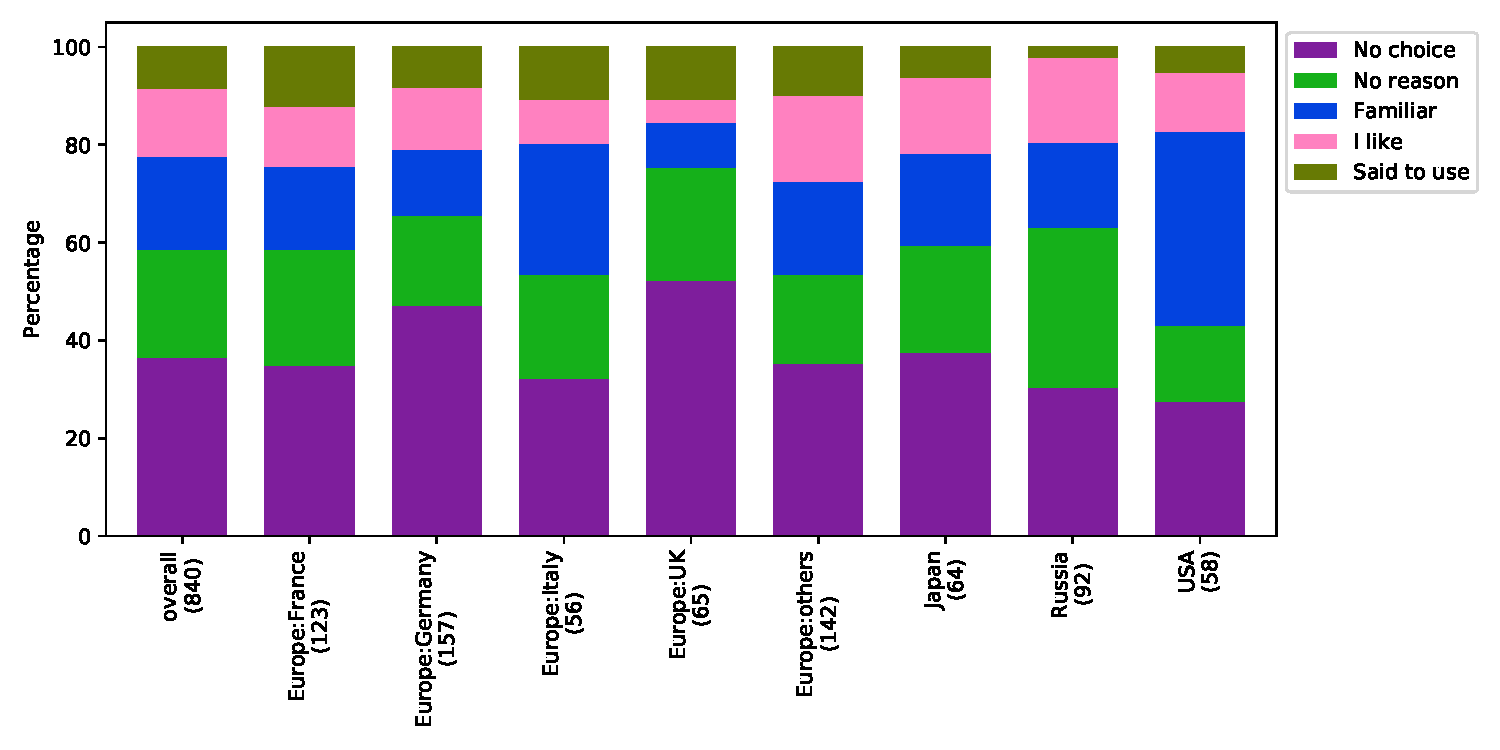
\includegraphics[width=10cm]{../pdfs/Q13.pdf}
\caption{Simple analysis: Q13}
\label{fig:Q13}
\end{center}
\end{figure}
